% !TEX program = xelatex
\documentclass[UTF8,aspectratio=169,11pt,fontset=none]{ctexbeamer}

\usepackage{fontspec}
\usepackage{amsmath,amssymb}
\usepackage{booktabs,tabularx,array}
\usepackage{graphicx}
\usepackage{tikz}
\usetikzlibrary{arrows.meta,positioning}

\setmainfont{TeX Gyre Termes}
\setsansfont{TeX Gyre Heros}
\setmonofont{TeX Gyre Cursor}
\setCJKmainfont{FandolSong-Regular.otf}[
  BoldFont=FandolSong-Bold.otf,
  ItalicFont=FandolKai-Regular.otf
]
\setCJKsansfont{FandolHei-Regular.otf}[
  BoldFont=FandolHei-Bold.otf
]
\setCJKmonofont{FandolSong-Regular.otf}
\ctexset{
  section/format=\Large\sffamily\bfseries,
  subsection/format=\large\sffamily\bfseries
}

% Structural colors are grayscale on purpose. Saturated colors are reserved
% for the measured data figures.
\definecolor{navy}{HTML}{202020}
\definecolor{blue}{HTML}{4A4A4A}
\definecolor{teal}{HTML}{5F5F5F}
\definecolor{coral}{HTML}{5F5F5F}
\definecolor{amber}{HTML}{5F5F5F}
\definecolor{ink}{HTML}{151515}
\definecolor{muted}{HTML}{666666}
\definecolor{paleblue}{HTML}{F4F4F4}
\definecolor{paleteal}{HTML}{F4F4F4}
\definecolor{paleamber}{HTML}{F4F4F4}
\definecolor{palecoral}{HTML}{F4F4F4}
\definecolor{linegray}{HTML}{B9B9B9}

\setbeamertemplate{navigation symbols}{}
\setbeamercolor{normal text}{fg=ink,bg=white}
\setbeamercolor{structure}{fg=ink}
\setbeamercolor{frametitle}{fg=ink,bg=white}
\setbeamercolor{block title}{fg=ink,bg=white}
\setbeamercolor{block body}{fg=ink,bg=white}
\setbeamerfont{frametitle}{size=\large,series=\bfseries}
\setbeamerfont{normal text}{size=\normalsize}
\setbeamertemplate{itemize item}{\textcolor{black!70}{\small\textbullet}}
\setbeamertemplate{itemize subitem}{\textcolor{black!55}{\scriptsize--}}
\setbeamertemplate{caption}[numbered]

\setbeamertemplate{frametitle}{%
  \vskip0.08cm
  \hspace{0.02cm}\insertframetitle
  \par\vskip0.12cm
}
\setbeamertemplate{footline}{%
  \hbox{%
    \begin{beamercolorbox}[wd=\paperwidth,ht=1.7ex,dp=0.5ex,
      leftskip=0.25cm,rightskip=0.25cm]{author in head/foot}%
      \hfill\textcolor{navy}{\scriptsize\insertframenumber/\inserttotalframenumber}\hfill
    \end{beamercolorbox}%
  }%
}
\setbeamersize{text margin left=0.20cm,text margin right=0.20cm}

\setbeamertemplate{block begin}{%
  \par\vskip0.30em%
  {\usebeamerfont*{block title}\bfseries\insertblocktitle}\par
  \vskip0.12em%
}
\setbeamertemplate{block end}{\vskip0.35em}
\setbeamertemplate{block alerted begin}{%
  \par\vskip0.30em%
  {\usebeamerfont*{block title}\bfseries\insertblocktitle}\par
  \vskip0.12em%
}
\setbeamertemplate{block alerted end}{\vskip0.35em}
\setbeamertemplate{block example begin}{%
  \par\vskip0.30em%
  {\usebeamerfont*{block title}\bfseries\insertblocktitle}\par
  \vskip0.12em%
}
\setbeamertemplate{block example end}{\vskip0.35em}

\newcommand{\code}[1]{\nolinkurl{#1}}
\newcommand{\metric}[2]{%
  \begin{minipage}[t]{0.98\linewidth}\centering
    {\Large\bfseries #1}\par\vspace{0.02em}
    {\small #2}
  \end{minipage}%
}
\newcolumntype{L}[1]{>{\raggedright\arraybackslash}p{#1}}

\title[High-Performance MultiGrid]{High-Performance Implementation of\\
Multigrid Solver for Lattice QCD}
\subtitle{Clover--Wilson 传播子 · Strict MultiGrid · CUDA--C++}
\author[张鑫]{张鑫\\中国科学院近代物理研究所}
\date{2026-10-11 15:05--15:20}

\begin{document}

\begin{frame}[plain]
  \vspace{0.2cm}
  {\usebeamerfont{title}\usebeamercolor[fg]{title}
  \LARGE\bfseries High-Performance Implementation of\\
  Multigrid Solver for Lattice QCD\par}
  \vspace{0.45cm}
  {\large 面向 Lattice QCD 传播子求解的高性能多重网格实现\par}
  \vspace{0.9cm}
  \begin{columns}[T]
    \begin{column}{0.42\textwidth}
      \textbf{汇报人}\quad 张鑫\\
      中国科学院近代物理研究所\\
      2026-10-11 15:05--15:20
    \end{column}
    \begin{column}{0.52\textwidth}
      \textbf{项目}\quad \url{https://github.com/zhangxin8069/PyQCU}\\
      \textbf{镜像}\quad \url{https://gitee.com/zhangxin8069/PyQCU}\\
      \textbf{文档}\quad \url{https://gitee.com/zhangxin8069/PyQCU/tree/main/docs}\\
      \textbf{日志}\quad \url{https://gitee.com/zhangxin8069/PyQCU/tags}
    \end{column}
  \end{columns}
  \vfill
  \centering
  \small 性能结论统一采用 \texttt{git tag test27}：66 个精确单元、132 条 side record
\end{frame}

\section{传播子与 Dirac 算子}

\begin{frame}[t]{Wilson \& Clover: fine-level Dirac operator conventions}
\begin{columns}[T,totalwidth=\textwidth]
\begin{column}{0.48\textwidth}
  \begin{block}{Wilson Dslash}
  \footnotesize
  \begin{equation}\tag{1}
  \begin{aligned}
  (H\psi)_x
  &=\sum_{\mu=0}^{3}\Big[
  (1-\gamma_\mu)U_{x,\mu}\psi_{x+\hat\mu}\\
  &\quad +(1+\gamma_\mu)U^\dagger_{x-\hat\mu,\mu}\psi_{x-\hat\mu}\Big],\\
  D_W&=(m_0+4)I-\frac12H\\
  &=(m_0+4)(I-\kappa H),\\
  \kappa&=\frac{1}{2m_0+8}.
  \end{aligned}
  \end{equation}
  \end{block}
\end{column}
\begin{column}{0.48\textwidth}
  \begin{block}{Clover 改进（当前 \(u_0=1,c_{\rm sw}=1\)）}
  \small
  \[
  Q_{\mu\nu}=P_{\mu\nu}+P_{\nu,-\mu}
  +P_{-\mu,-\nu}+P_{-\nu,\mu}
  \]
  \[
  C_{\mu\nu}=Q_{\mu\nu}-Q^\dagger_{\mu\nu}
  \]
  \begin{equation}\tag{2}
  T_p=-\frac{\kappa c_{\rm sw}}{8u_0}
  \sum_{\mu<\nu}\gamma_\mu\gamma_\nu C_{\mu\nu}
  \end{equation}
  \[
  A_p=I_p+T_p
  \]
  \end{block}
\end{column}
\end{columns}
\vspace{-0.45cm}
\end{frame}

\begin{frame}[t]{Raw Dslash: eight-neighbor matrix-free stencil}
\begin{columns}[T,totalwidth=\textwidth]
\begin{column}{0.47\textwidth}
  \begin{block}{Kernel flow / entry semantics}
  \small
  \begin{itemize}
    \item Per site: four forward and four backward neighbors；
    \item \(1\pm\gamma_\mu\): four-spinor \(\to\) two components；
    \item \(SU(3)\) transport and eight-direction accumulation。
  \end{itemize}
  \end{block}
  \small
  原始入口返回裸核 \(H\)；带单位项入口返回
  \(I-(\kappa/u_0)H\)。
\end{column}
\begin{column}{0.49\textwidth}
  \begin{center}
  \begin{tikzpicture}[
    node distance=2.5mm,
    box/.style={draw=none,fill=none,
      align=center,minimum width=2.8cm,minimum height=0.66cm,font=\small},
    arrow/.style={-{Latex[length=2mm]},draw=black,line width=0.7pt}
  ]
    \node[box] (n) {邻居旋量读取};
    \node[box,below=of n] (p) {\(1\pm\gamma_\mu\) 投影};
    \node[box,below=of p] (u) {\(SU(3)\) 平移};
    \node[box,below=of u] (a) {八方向累加};
    \draw[arrow] (n)--(p);\draw[arrow] (p)--(u);\draw[arrow] (u)--(a);
  \end{tikzpicture}
  \end{center}
  \begin{minipage}{0.96\linewidth}
  \small
  \textbf{性能本质：}最近邻模板天然 bandwidth-bound；
  \(4\to2\) spin projection、\(SU(3)\) 重用和尾置时空维决定有效带宽。
  \end{minipage}
\end{column}
\end{columns}
\end{frame}

\begin{frame}[t,shrink=5]{Even--odd Schur: half-size outer Krylov problem}
\begin{columns}[T,totalwidth=\textwidth]
\begin{column}{0.46\textwidth}
  \begin{block}{Block matrix and Schur complement}
  \small
  \begin{equation}\tag{3}
  D_{\rm pc}=
  \begin{pmatrix}
  A_e&-\kappa H_{eo}\\
  -\kappa H_{oe}&A_o
  \end{pmatrix}
  \end{equation}
  \begin{equation}\tag{4}
  S_o=A_o-\kappa^2H_{oe}A_e^{-1}H_{eo}
  \end{equation}
  \end{block}
  \begin{block}{Solve and reconstruct}
  \small
  \begin{equation}\tag{5}
  b_o^{\rm pc}=b_o+\kappa H_{oe}A_e^{-1}b_e
  \end{equation}
  \begin{equation}\tag{6}
  S_ox_o=b_o^{\rm pc}
  \end{equation}
  \begin{equation}\tag{7}
  x_e=A_e^{-1}(b_e+\kappa H_{eo}x_o)
  \end{equation}
  \end{block}
\end{column}
\begin{column}{0.50\textwidth}
  \begin{center}
  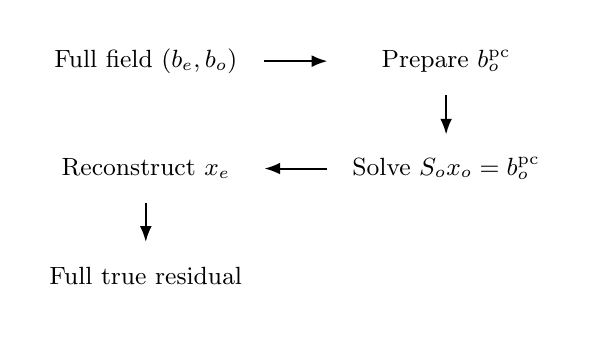
\begin{tikzpicture}[
    node distance=5mm and 8mm,
    box/.style={draw=none,fill=none,
      align=center,minimum width=3.0cm,minimum height=0.85cm,font=\small},
    arrow/.style={-{Latex[length=2mm]},draw=black,line width=0.7pt}
  ]
    \node[box] (full) {Full field \((b_e,b_o)\)};
    \node[box,right=of full] (prep) {Prepare \(b_o^{\rm pc}\)};
    \node[box,below=of prep] (solve) {Solve \(S_ox_o=b_o^{\rm pc}\)};
    \node[box,left=of solve] (rec) {Reconstruct \(x_e\)};
    \node[box,below=of rec] (res) {Full true residual};
    \draw[arrow] (full)--(prep);
    \draw[arrow] (prep)--(solve);
    \draw[arrow] (solve)--(rec);
    \draw[arrow] (rec)--(res);
  \end{tikzpicture}
  \end{center}
\end{column}
\end{columns}
\end{frame}

\section{MultiGrid 算法}

\begin{frame}[t,shrink=5]{MultiGrid: null-space coarse space + smoother}
\begin{columns}[T,totalwidth=\textwidth]
\begin{column}{0.48\textwidth}
  \begin{block}{Four core objects}
  \normalsize
  \begin{itemize}
    \item 近零模：\(A_lB_l\approx0\)
    \item 局部正交：\(P_l^\dagger P_l=I\)
    \item 转移对：\(R_l=P_l^\dagger\)
    \item Galerkin 粗算子：
      \(A_{l+1}=R_lA_lP_l\)
  \end{itemize}
  \end{block}
  \normalsize
  \vspace{0.35cm}
  \begin{equation}\tag{8}
  e=e_{\rm high}+e_{\rm low},\qquad
  A_lB_l\approx0
  \end{equation}
\end{column}
\begin{column}{0.49\textwidth}
  \begin{center}
  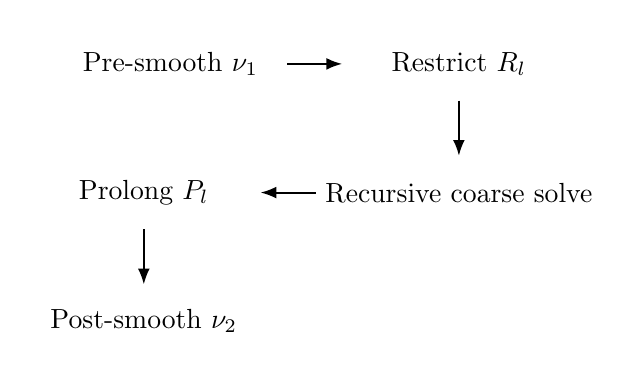
\begin{tikzpicture}[
    node distance=7mm,
    box/.style={draw=none,fill=none,
      align=center,minimum width=2.95cm,minimum height=0.92cm,font=\normalsize},
    arrow/.style={-{Latex[length=2mm]},draw=black,line width=0.7pt}
  ]
    \node[box] (pre) {Pre-smooth \(\nu_1\)};
    \node[box,right=of pre] (r) {Restrict \(R_l\)};
    \node[box,below=of r] (c) {Recursive coarse solve};
    \node[box,left=of c] (p) {Prolong \(P_l\)};
    \node[box,below=of p] (post) {Post-smooth \(\nu_2\)};
    \draw[arrow] (pre)--(r);
    \draw[arrow] (r)--(c);
    \draw[arrow] (c)--(p);
    \draw[arrow] (p)--(post);
  \end{tikzpicture}
  \end{center}
\end{column}
\end{columns}
\end{frame}

\begin{frame}[t,shrink=5]{Null-vector construction: inexact inverse correction + local QR}
\begin{columns}[T,totalwidth=\textwidth]
\begin{column}{0.56\textwidth}
  \begin{center}
  \textbf{Algorithm 1}\quad Null-vector construction
  \end{center}
  \fontsize{9}{11}\selectfont
  \begin{tabular}{@{}>{\raggedright\arraybackslash}p{0.96\linewidth}@{}}
  \toprule
  \(\mathbf{Input:}\;A_l,e_l,n_v,b,n_{\rm iter}{=}2,
    \varepsilon_{\rm rtol}{=}10^{-2},\mathrm{seed}{=}42\)\\
  \(\mathbf{for}\;j=1,\ldots,n_v\)\\
  \(\quad v_j\sim\mathcal N(0,I)\)\\
  \(\quad\mathbf{repeat}\;n_{\rm iter}\)\\
  \(\quad\quad x_j\approx
    \operatorname{solve}_{\rm rel}(A_lx=A_lv_j;\varepsilon_{\rm rtol})\)\\
  \(\quad\quad v_j\leftarrow v_j-x_j\)\\
  \(\quad v_j\leftarrow v_j/\|v_j\|_2\)\\
  \(\mathbf{for\;aggregate}\;c\)\\
  \(\quad V_c=[v_j]_{j\in c};\quad
    Q_cR_c=\operatorname{reducedQR}(V_c)\)\\
  \(\quad P_l|_c\leftarrow Q_c;\quad
    \operatorname{cache\;blocked}\;P_l,V_l\)\\
  \(R_l\leftarrow P_l^\dagger;\quad
    D_{l+1}\leftarrow R_lD_lP_l\)\\
  \bottomrule
  \end{tabular}
\end{column}
\begin{column}{0.42\textwidth}
  \small
  \begin{equation}\tag{9}
  \begin{aligned}
  x_j&\approx A_l^{-1}(A_lv_j),\\
  v_j&\leftarrow v_j-x_j,\qquad
  v_j\leftarrow v_j/\|v_j\|_2
  \end{aligned}
  \end{equation}
  \begin{equation}\tag{10}
  \begin{aligned}
  V_c&=P_cR_c,\qquad E=2n_v\\
  P_c^\dagger P_c&=I_E
  \end{aligned}
  \end{equation}
  \begin{equation}\tag{11}
  \begin{aligned}
  (R_lv)_X&=\sum_{x\in\mathcal A_X}V_X^\dagger v(x)\\
  (P_lz)(x)&=V_Xz(X)
  \end{aligned}
  \end{equation}
  \begin{equation}\tag{12}
  A_{l+1}=R_lA_lP_l,\qquad R_l=P_l^\dagger
  \end{equation}
  \small
  \textbf{关键实现：}相对容差、独立 RNG seed、分块 batched solve；
  threaded path 支持 breakdown/NaN 重采样，batch path 当前没有逐向量重试。
  \par\vspace{0.15em}
  \textbf{路径区分：}\code{local\_orthogonalize} 使用 batched reduced QR；
  Strict/reference 的 aggregate CGS 是另一条实现，不能混写。
\end{column}
\end{columns}
\end{frame}

\begin{frame}[t]{Preconditioned Bi-CGStab for coarse solves}
\begin{columns}[T,totalwidth=\textwidth]
\begin{column}{0.49\textwidth}
  \begin{center}
  \textbf{Algorithm 2}\quad Preconditioned Bi-CGStab
  \end{center}
  \fontsize{11}{13}\selectfont
  \begin{tabular}{@{}>{\raggedright\arraybackslash}p{0.96\linewidth}@{}}
  \toprule
  \(r^{(0)}=b-Ax^{(0)}\)\\
  \(\tilde r=r^{(0)}\)\\
  \(\mathbf{for}\;i=1,2,\ldots\)\\
  \(\quad\rho_{i-1}=\tilde r^\dagger r^{(i-1)};\;
    \mathbf{if}\;\rho_{i-1}=0\;\mathbf{fail}\)\\
  \(\quad\mathbf{if}\;i=1\;\mathbf{then}\;
    p^{(1)}=r^{(0)}\)\\
  \(\quad\mathbf{else}\)\\
  \(\quad\quad\beta_{i-1}=
    \dfrac{\alpha_{i-1}\rho_{i-1}}
    {\omega_{i-1}\rho_{i-2}}\)\\
  \(\quad\quad p^{(i)}=r^{(i-1)}
    +\beta_{i-1}(p^{(i-1)}-\omega_{i-1}v^{(i-1)})\)\\
  \(\quad\text{solve }M\hat p=p^{(i)};\quad v^{(i)}=A\hat p\)\\
  \bottomrule
  \end{tabular}
\end{column}
\begin{column}{0.49\textwidth}
  \vspace{0.62cm}
  \fontsize{10}{12}\selectfont
  \begin{tabular}{@{}>{\raggedright\arraybackslash}p{0.96\linewidth}@{}}
  \toprule
  \(\quad\alpha_i=\rho_{i-1}/
    (\tilde r^\dagger v^{(i)})\)\\
  \(\quad s=r^{(i-1)}-\alpha_i v^{(i)}\)\\
  \(\quad\mathbf{if}\;\|s\|/\|b\|\le\varepsilon\;\mathbf{then}\;
    x^{(i)}=x^{(i-1)}+\alpha_i\hat p;
    \mathbf{stop}\)\\
  \(\quad\text{solve }M\hat s=s;\quad t=A\hat s\)\\
  \(\quad\omega_i=t^\dagger s/(t^\dagger t)\)\\
  \(\quad r^{(i)}=s-\omega_i t\)\\
  \(\quad x^{(i)}=x^{(i-1)}
    +\alpha_i\hat p+\omega_i\hat s\)\\
  \(\mathbf{end\,for}\)\\
  \bottomrule
  \end{tabular}
\end{column}
\end{columns}
\end{frame}

\section{PyQCU Strict 实现}

\begin{frame}[t,shrink=7]{Strict path: \(D=X+H\) and full-coarse assets}
\begin{columns}[T,totalwidth=\textwidth]
\begin{column}{0.49\textwidth}
  \begin{block}{Level decomposition}
  \normalsize
  \begin{equation}\tag{13}
  \begin{aligned}
    D_l&=X_l+H_l\\
    \widehat D_l&=X_l^{-1}D_l\\
    D_{l+1}&=R_l\widehat D_lP_l
  \end{aligned}
  \end{equation}
  \begin{equation}\tag{14}
  \mathcal G_l=\{
  V_l,X_{l+1},X_{l+1}^{-1},
  Y_{l+1}^{\rm f/b},\widehat Y_{l+1}^{\rm f/b}\}
  \end{equation}
  \end{block}
  \begin{minipage}{0.96\linewidth}
  \normalsize
  Runtime assets: \(X,X^{-1},Y^{\rm f/b},\widehat Y^{\rm f/b},V\)。
  Coarse levels keep full geometry; fine level uses compact target parity.
  \end{minipage}
\end{column}
\begin{column}{0.49\textwidth}
  \begin{center}
  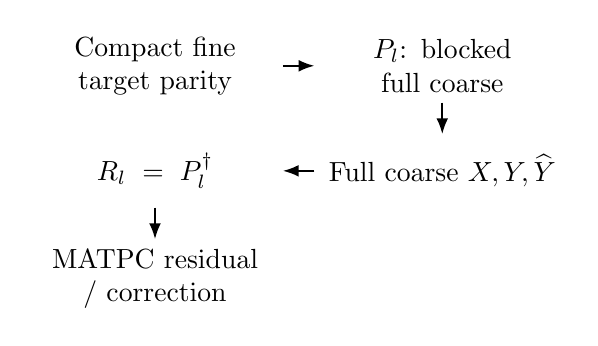
\begin{tikzpicture}[
    node distance=4mm,
    box/.style={draw=none,fill=none,
      align=center,text width=3.0cm,minimum height=0.92cm,font=\normalsize},
    arrow/.style={-{Latex[length=2mm]},draw=black,line width=0.7pt}
  ]
    \node[box] (fine) {Compact fine target parity};
    \node[box,right=of fine] (p) {\(P_l\): blocked full coarse};
    \node[box,below=of p] (asset) {Full coarse \(X,Y,\widehat Y\)};
    \node[box,left=of asset] (r) {\(R_l=P_l^\dagger\)};
    \node[box,below=of r] (res) {MATPC residual / correction};
    \draw[arrow] (fine)--(p);
    \draw[arrow] (p)--(asset);
    \draw[arrow] (asset)--(r);
    \draw[arrow] (r)--(res);
  \end{tikzpicture}
  \end{center}
\end{column}
\end{columns}
\end{frame}

\begin{frame}[t,shrink=6]{Coarse \(X/Y\): onsite, directional links and \(\widehat Y\)}
\begin{columns}[T,totalwidth=\textwidth]
\begin{column}{0.49\textwidth}
  \begin{block}{Construction of \(X\) and \(Y\)}
  \small
  \begin{equation}\tag{15}
  E=2n_v,\qquad X_\ell,Y^{\rm f/b}_{\ell,\mu}
  \in\mathbb C^{E\times E}
  \end{equation}
  \begin{equation}\tag{16}
  X_C(X)=\sum_{x\in\mathcal A_X}V_X^\dagger C V_X
  \end{equation}
  \begin{equation}\tag{17}
  Y^{\rm f}_{\mu}(X)=-\kappa\sum_{x\in\mathcal A_X}
  (AV_X)^\dagger U_\mu V_{X+\hat\mu}
  \end{equation}
  \begin{equation}\tag{18}
  Y^{\rm b}_{\mu}(X-\hat\mu)=-\kappa\sum_{x\in\mathcal A_X}
  V_X^\dagger U^\dagger_\mu AV_{X-\hat\mu}
  \end{equation}
  \(AV=C^{-1}V\)（Clover-PC）；raw path 取 \(AV=V\)。
  \end{block}
\end{column}
\begin{column}{0.49\textwidth}
  \begin{block}{Raw action and preconditioned links}
  \small
  \begin{equation}\tag{19}
  \begin{aligned}
  D_cz(X)&=X(X)z(X)\\
  &+\sum_\mu\left[Y_\mu^{\rm f}(X)z(X+\hat\mu)
  +Y_\mu^{\rm b}(X-\hat\mu)^\dagger z(X-\hat\mu)\right]
  \end{aligned}
  \end{equation}
  \begin{equation}\tag{20}
  \widehat Y^{\rm f}_{\mu}(X)=X^{-1}(X)Y^{\rm f}_{\mu}(X)
  \end{equation}
  \begin{equation}\tag{21}
  \widehat Y^{\rm b}_{\mu}(X-\hat\mu)
  =Y^{\rm b}_{\mu}(X-\hat\mu)X^{-\dagger}(X)
  \end{equation}
  \begin{equation}\tag{22}
  M_p^cx_p=x_p-\widehat H_{pq}\widehat H_{qp}x_p
  \end{equation}
  \begin{equation}\tag{23}
  \widehat Hz=\sum_\mu\left[
  \widehat Y_\mu^{\rm f}(X)z(X+\hat\mu)
  +\widehat Y_\mu^{\rm b}(X-\hat\mu)^\dagger z(X-\hat\mu)
  \right]
  \end{equation}
  \end{block}
\end{column}
\end{columns}
\vspace{-0.15cm}
\begin{minipage}{0.96\textwidth}
\small
PC dslash 只应用 \(\widehat Y\) hopping；backward 使用
\(X-\hat\mu\) 的 storage block，左右矩阵顺序不可交换。
\end{minipage}
\end{frame}

\begin{frame}[t,shrink=10]{V-cycle inside, flexible FGMRES outside}
\begin{columns}[T,totalwidth=\textwidth]
\begin{column}{0.49\textwidth}
  \begin{center}\textbf{Algorithm 3}\quad Recursive MG preconditioner\end{center}
  \begin{tabular}{@{}>{\raggedright\arraybackslash}p{0.96\linewidth}@{}}
  \toprule
  \(\mathbf{Input:}\;A_l,r_l,
    \{S_{\rm pre},S_{\rm post},P_l,R_l\}\)\\
  \(\mathbf{if}\;l=L-1\;\mathbf{then}\;
    z_l\gets A_l^{-1}r_l\)\\
  \(\mathbf{else}\)\\
  \(\quad y_l\gets S_{\rm pre}^{\nu_1}(r_l)\)\\
  \(\quad r_{l+1}\gets R_l(r_l-A_l y_l)\)\\
  \(\quad e_{l+1}\gets M_{l+1}^{-1}r_{l+1}\)\\
  \(\quad z_l\gets y_l+P_l e_{l+1}\)\\
  \(\quad z_l\gets S_{\rm post}^{\nu_2}(z_l)\)\\
  \(\mathbf{end\,if}\)\\
  \bottomrule
  \end{tabular}
  \vspace{0.3cm}
  \begin{equation}\tag{24}
  x^{(k+1)}=x^{(k)}+z^{(k)}
  \end{equation}
  \begin{equation}\tag{25}
  z_l=S_{\rm post}^{\nu_2}\left[
  S_{\rm pre}^{\nu_1}r_l+
  P_lM_{l+1}^{-1}R_l
  (r_l-A_lS_{\rm pre}^{\nu_1}r_l)
  \right]
  \end{equation}
\end{column}
\begin{column}{0.49\textwidth}
  \begin{center}\textbf{Algorithm 4}\quad Flexible FGMRES\end{center}
  \begin{tabular}{@{}>{\raggedright\arraybackslash}p{0.96\linewidth}@{}}
  \toprule
  \(r_0=b-Ax^{(0)},\;v_1=r_0/\|r_0\|\)\\
  \(\mathbf{for}\;j=1,\ldots,m\)\\
  \(\quad z_j=M^{-1}v_j;\quad w=Az_j\)\\
  \(\quad \mathbf{for}\;i=1,\ldots,j\)\\
  \(\quad\quad h_{ij}=v_i^\dagger w;\quad
    w=w-h_{ij}v_i\)\\
  \(\quad \mathbf{end\,for}\)\\
  \(\quad h_{j+1,j}=\|w\|;\quad
    v_{j+1}=w/h_{j+1,j}\)\\
  \(\quad \text{apply Givens rotations to }H_j\)\\
  \(\mathbf{end\,for}\)\\
  \(x^{(k+1)}=x^{(k)}+Z_jy\)\\
  \bottomrule
  \end{tabular}
\end{column}
\end{columns}
\end{frame}

\begin{frame}[t,shrink=4]{CUDA--C++ execution path: fine kernel, coarse latency, MPI overlap}
\begin{columns}[T,totalwidth=\textwidth]
\begin{column}{0.55\textwidth}
\begin{center}\textbf{Algorithm 5}\quad Distributed PyQCU MG call path\end{center}
\small
\begin{tabular}{@{}>{\raggedright\arraybackslash}p{0.96\linewidth}@{}}
\toprule
\(\mathbf{Input:}\;b_p,A_l,\{V_l,X_l,Y_l,\widehat Y_l\},p\)\\
\textbf{1.} partition: rank-local / send / inside / receive\\
\textbf{2.} fine Dslash: \(1\pm\gamma_\mu\) projection \(\to\) \(SU(3)\) transport\\
\textbf{3.} coarse hop: \(X\) onsite + \(\widehat Y\) forward/backward links\\
\textbf{4.} V-cycle: pre-smooth, restrict, recurse, prolong, post-smooth\\
\textbf{5.} outer FGMRES: Arnoldi + frozen/updated coarse hierarchy\\
\textbf{6.} correction: receive halo, add remote correction, true residual\\
\bottomrule
\end{tabular}
\end{column}
\begin{column}{0.43\textwidth}
\small
\begin{tabular}{@{}p{0.25\linewidth}p{0.66\linewidth}@{}}
\toprule
hot path & optimization\\
\midrule
fine kernel & 4\(\to\)2 spin projection; \(SU(3)\) reuse; \(xyzt\) coalescing\\
coarse apply & 33-point stencil; device scalar; fused \(X\)-\(\widehat Y\) update\\
Krylov & fused dot/vector update; CUDA Graph; smallest-level solve\\
setup & batched reduced QR; colored Galerkin; workspace cap\\
MPI & 32-slot coarse halo; nonblocking vector halo; cached link halo; remote correction\\
cache & persistent hierarchy; HDF5 P/V/\(X/Y\); schema/hash validation\\
\bottomrule
\end{tabular}
\end{column}
\end{columns}
\end{frame}

\begin{frame}[t,shrink=3]{CUDA--C++ internals: persistent state, fused recurrences, overlap boundary}
\begin{columns}[T,totalwidth=\textwidth]
\begin{column}{0.52\textwidth}
\begin{center}\textbf{Algorithm 6}\quad Strict fused execution schedule\end{center}
\small
\begin{tabular}{@{}>{\raggedright\arraybackslash}p{0.96\linewidth}@{}}
\toprule
\textbf{1.} compact fine parity: \(b_p\mapsto b_p^{\rm pc}\)\\
\textbf{2.} MATPC: \(x_p\leftarrow x_p-\widehat H_{pq}\widehat H_{qp}x_p\)\\
\textbf{3.} V-cycle: MR pre \(\to R_l\to\) coarse solve
\(\to P_l\to A_lr_l\to\) MR post\\
\textbf{4.} right FGMRES: \(z_j=\mathcal M^{-1}v_j,\;w=M_pz_j\);
Arnoldi; restart true residual\\
\textbf{5.} halo: local base \(\to\) post Irecv/Isend \(\to\) wait
\(\to\) unpack \(\to\) remote correction\\
\textbf{6.} cache: blocked \(P/V/X/Y\); HDF5 shape/dtype/hash validation\\
\bottomrule
\end{tabular}
\end{column}
\begin{column}{0.46\textwidth}
\footnotesize
\begin{tabular}{@{}p{0.24\linewidth}p{0.69\linewidth}@{}}
\toprule
mechanism & implementation detail\\
\midrule
fine Dslash & \(1\pm\gamma_\mu\): 4\(\to\)2 projection; \(SU(3)\) reuse; \(xyzt\) coalescing\\
coarse latency & device scalar; fused \(\beta/\rho\) and \(r/x\); adaptive dot reduction\\
graphs & segment replay for legacy kernels; cooperative coarsest solve; safe fallback\\
persistent state & preallocated streams/workspaces; hierarchy arena; FGMRES workspace\\
strict overlap & c64 nonblocking vector halo; c128 default off; link halo remains Sendrecv\\
setup/cache & colored/batched Galerkin; workspace cap; SHA256; atomic HDF5 publish\\
\bottomrule
\end{tabular}
\end{column}
\end{columns}
\end{frame}

\section{性能对照}

\begin{frame}[t,shrink=6]{QUDA comparison protocol: 66 exact units, 132 side records}
  \centering
  \small
  \begin{tabular}{@{}lllll@{}}
  \toprule
  device & precision & solvers & tracing & timing protocol\\
  \midrule
  V100 / P100\(\times2\) & c64 / c128 & BiCGStab / MG-2 / MG-3
  & on / off & 1 cold + 2 warmup + 5 steady\\
  \bottomrule
  \end{tabular}
  \par\vspace{0.14cm}
  66 distinct exact/effective combined units \(\cdot\) 132 side records
  \(\cdot\) 6 extra capacity substitutions
  \par\vspace{0.04cm}
  \(R=t_{\rm QUDA,steady}/t_{\rm PyQCU,steady}\) \(\cdot\) trace-off is formal
  \(\cdot\) test27 follows Strict MATPC + fused right-FGMRES
  \par\vspace{0.18cm}
  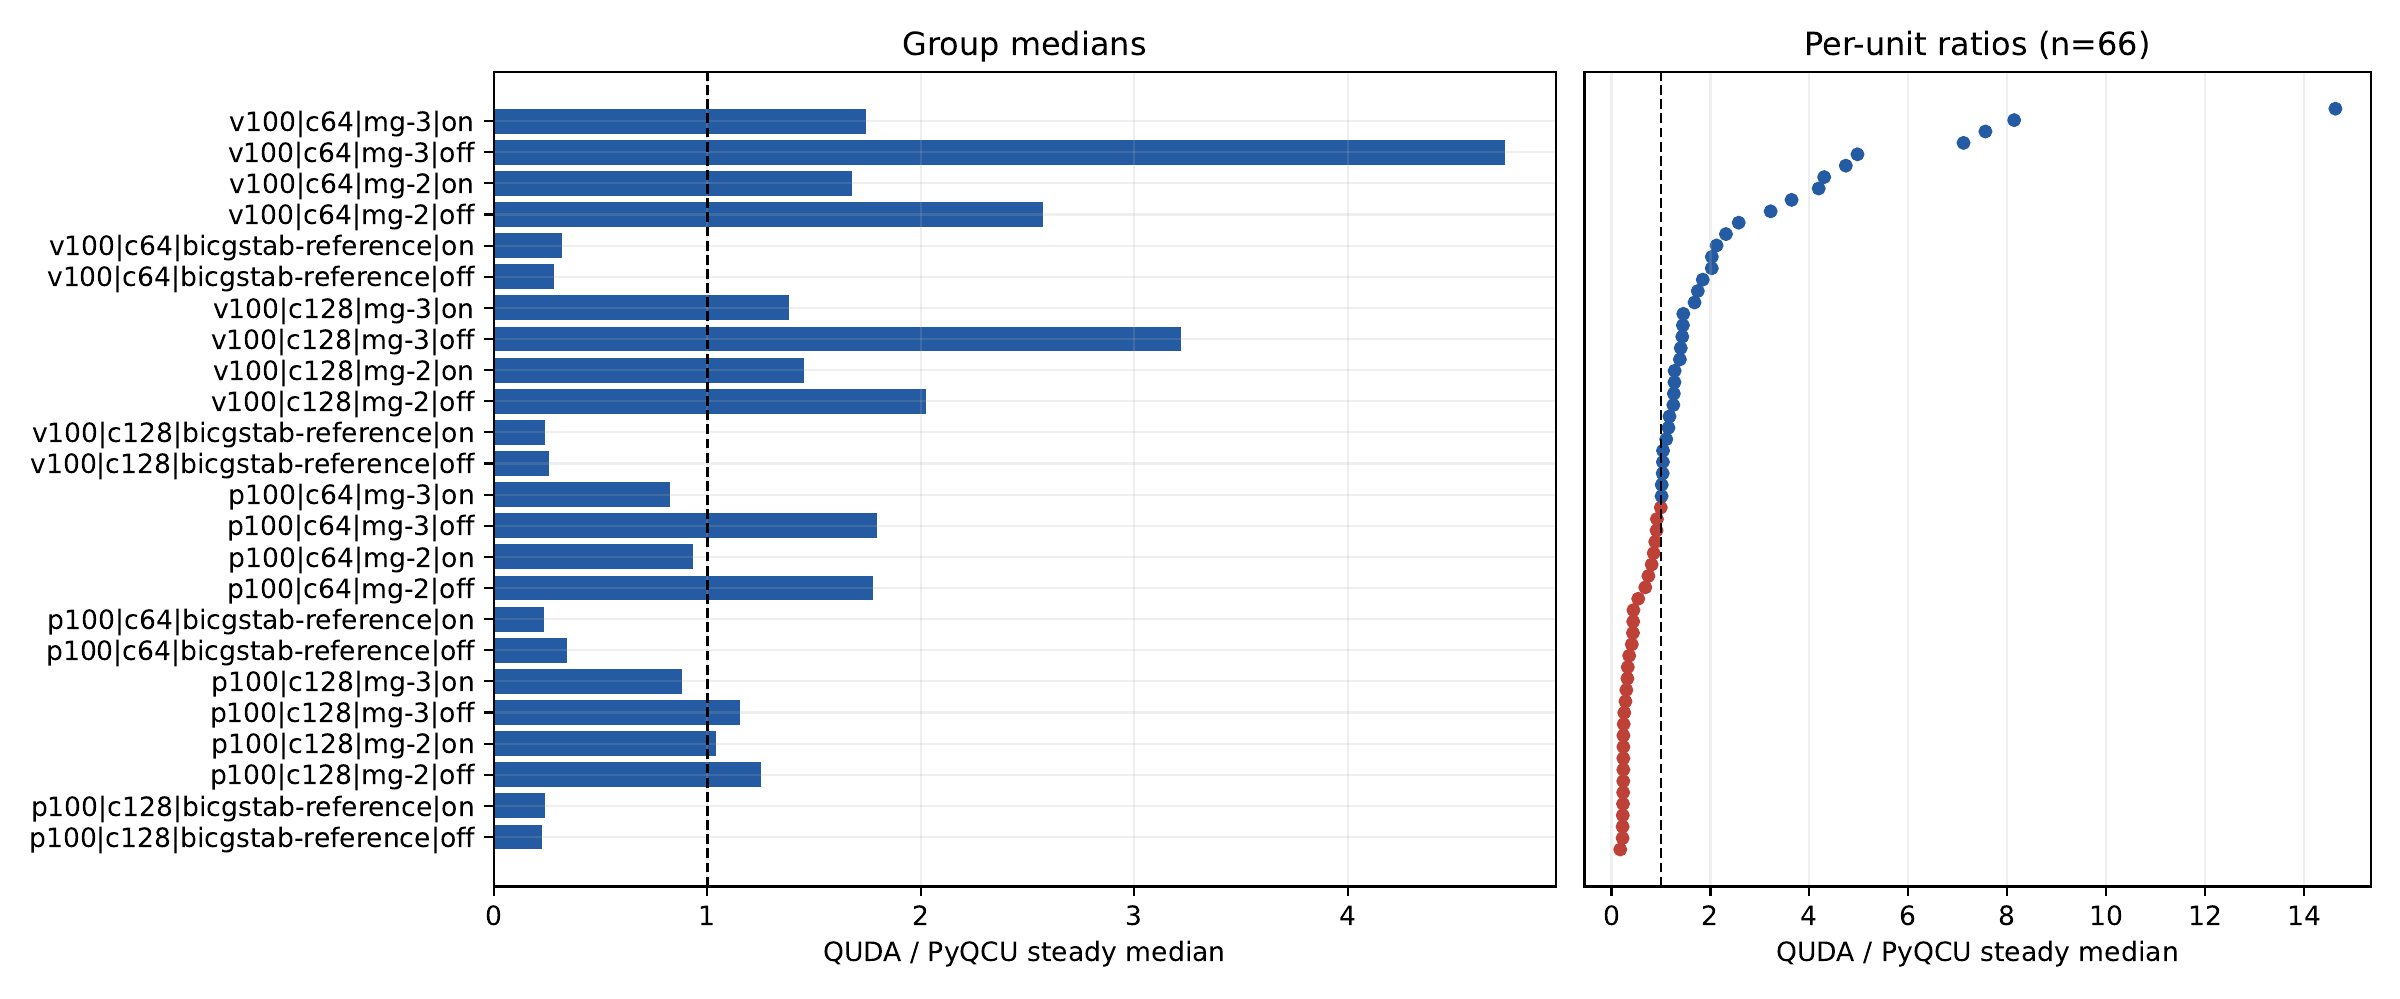
\includegraphics[width=0.99\textwidth,height=0.58\textheight,keepaspectratio]
  {High-Performance_Implementation_MG_assets/report_chart_assets/overlap_matrix.png}
  \par{\small 图 1：协议与 \(R\) 分布；替代项只作为容量与趋势证据，不进入原请求比值。}
\end{frame}

\begin{frame}[t,shrink=6]{Overall result: MG-specific gain, total median \(1.025\)}
  \centering
  \normalsize
  \(1.025=\operatorname{median}_{66}R\) \(\cdot\)
  \(35/44\) MG-2/3 with \(R>1\) (on/off) \(\cdot\)
  \(21/22\) trace-off MG \(\cdot\) \(0/22\) BiCGStab
  \(\cdot\) \(0.1766\)--\(14.63\) all-unit range
  \par\vspace{0.18cm}
  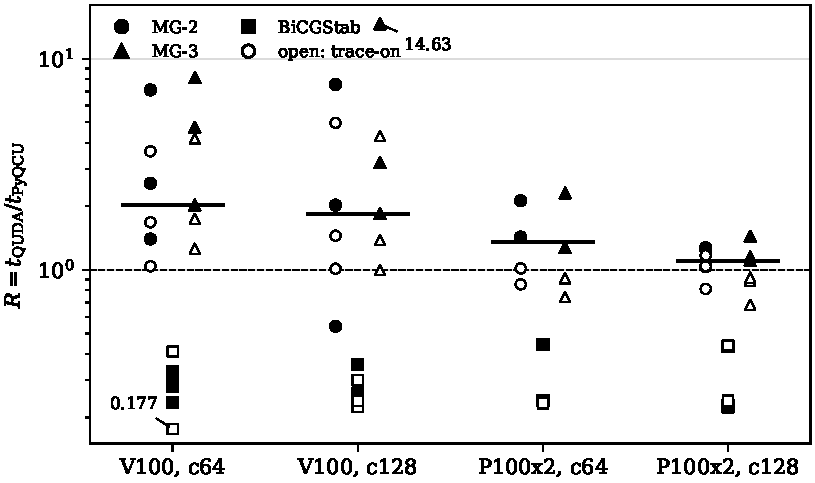
\includegraphics[width=0.98\textwidth,height=0.72\textheight,keepaspectratio]
  {High-Performance_Implementation_MG_assets/paper_assets/fig_ratio_distribution.pdf}
  \par{\small 图 2：每个点是一个精确 unit，水平线为对应 trace-off 分组中位数。}
\end{frame}

\begin{frame}[t,shrink=5]{Device and precision trends: V100 strong, P100 moderate}
  \centering
  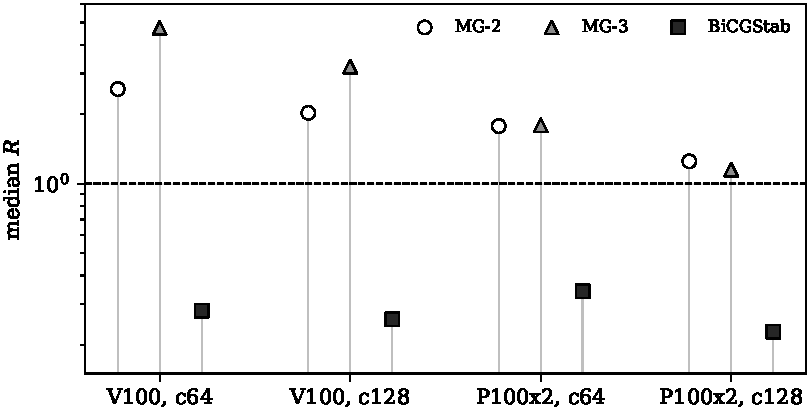
\includegraphics[width=0.99\textwidth,height=0.76\textheight,keepaspectratio]
  {High-Performance_Implementation_MG_assets/paper_assets/fig_group_medians.pdf}
  \par{\small 图 3：V100 c64/c128 MG-3 trace-off group medians
  \(4.74\times/3.22\times\)；P100\(\times2\) c64/c128 MG-2
  \(1.78\times/1.25\times\)。P100 c64 每组仅 \(n=2\)。}
\end{frame}

\begin{frame}[t,shrink=5]{trace-on stage attribution: coarse + other dominate}
  \centering
  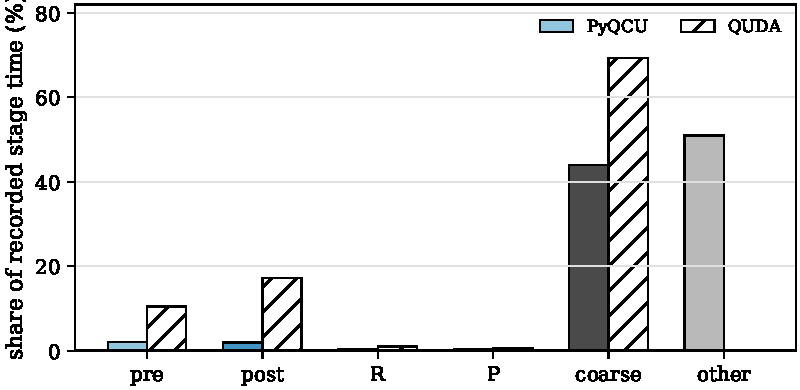
\includegraphics[width=0.99\textwidth,height=0.75\textheight,keepaspectratio]
  {High-Performance_Implementation_MG_assets/paper_assets/fig_stage_shares.pdf}
  \par{\small 图 4：逐 unit、逐侧阶段份额的中位数；PyQCU
  coarse \(+\) other \(\approx94.9\%\)，QUDA 具名 coarse \(\approx69.3\%\)。
  该量不是 wall-clock 总时间求和份额。}
\end{frame}

\begin{frame}[t,shrink=8]{device-wide memory and correctness gate}
  \begin{columns}[T,totalwidth=\textwidth]
  \begin{column}{0.58\textwidth}
    \centering
    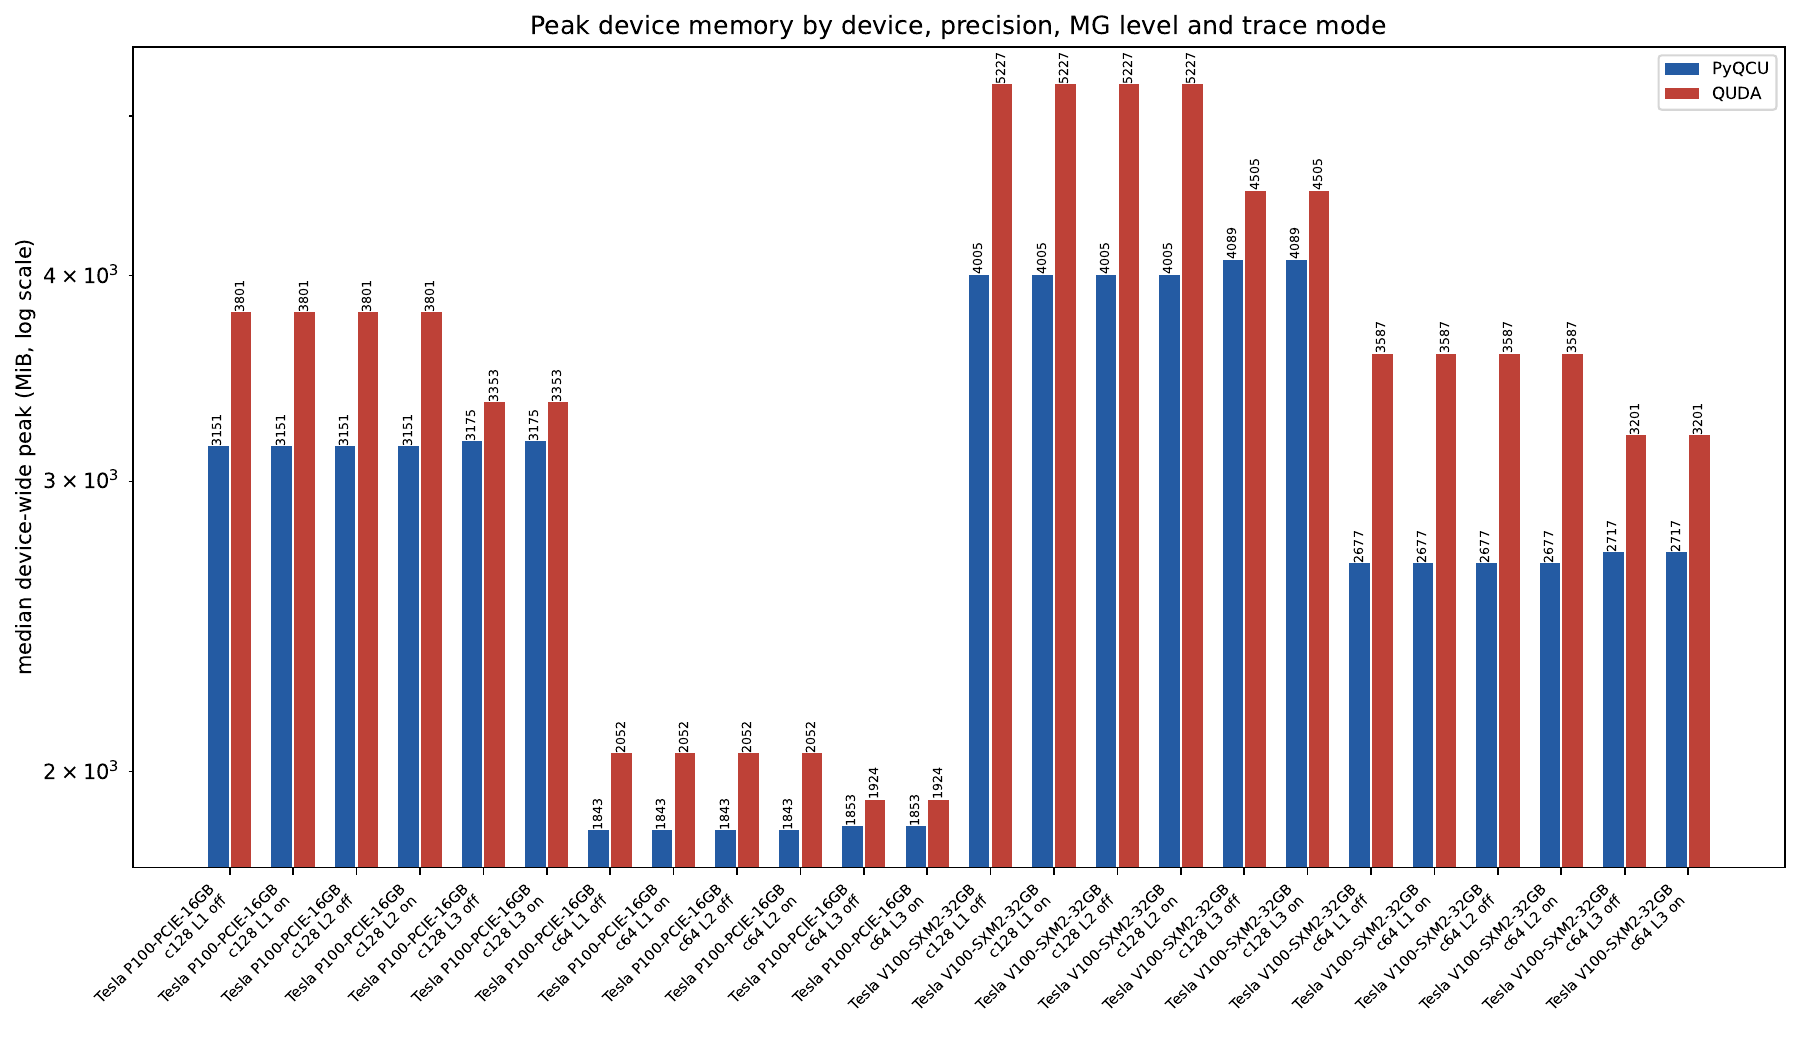
\includegraphics[width=\linewidth,height=0.61\textheight,keepaspectratio]
    {High-Performance_Implementation_MG_assets/report_chart_assets/mg_peak_memory.png}
    \par{\small 图 5：device-wide 观测峰值，不等同于单进程独占。}
  \end{column}
  \begin{column}{0.40\textwidth}
    \centering
    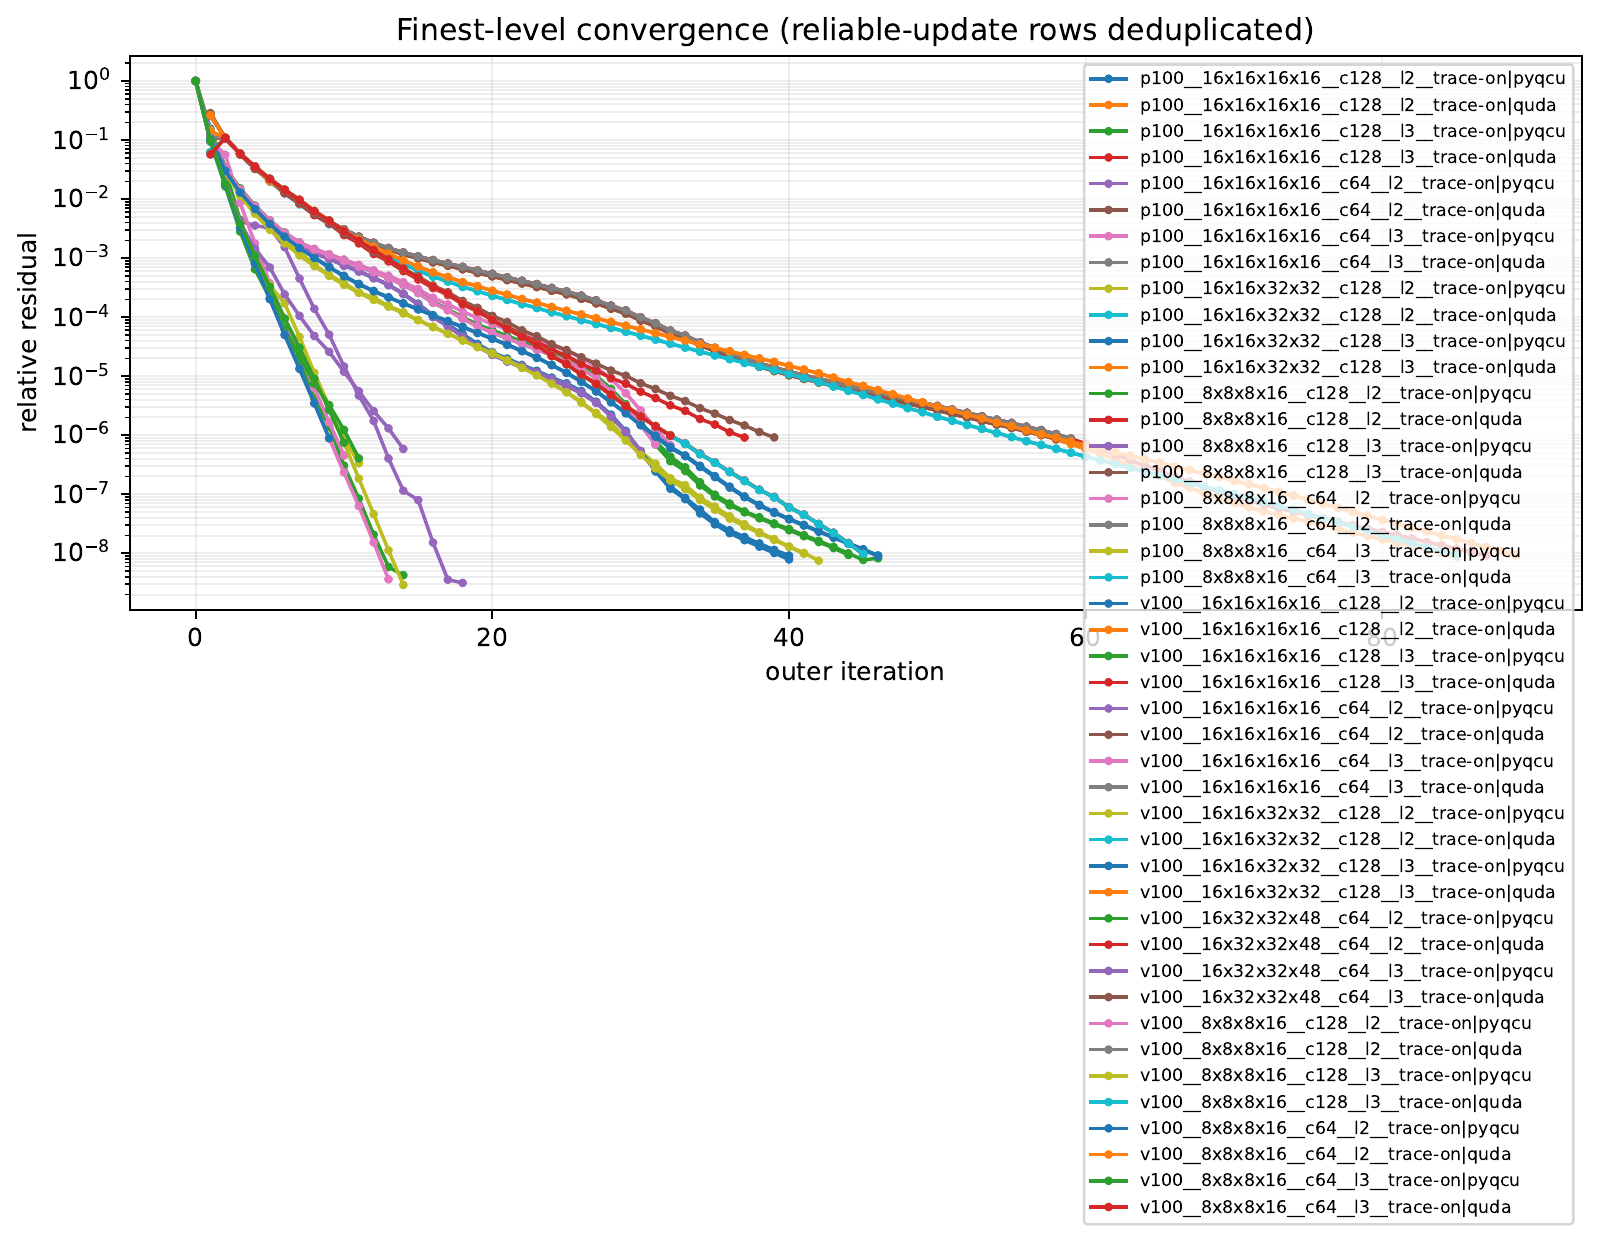
\includegraphics[width=\linewidth,height=0.40\textheight,keepaspectratio]
    {High-Performance_Implementation_MG_assets/report_chart_assets/mg_finest_residual.png}
    \par{\small 图 6：full-operator true residual；递推残差只用于趋势。}
    \par\vspace{0.18cm}
    \small 66 combined units:\\
    PyQCU full-operator true residual max \(7.4016\times10^{-7}\)\\
    QUDA max \(7.9721\times10^{-7}\)\\
    gate \(5\times10^{-6}\)\par
    \par\vspace{0.12cm}
    \footnotesize steady-phase device-wide max:\\
    PyQCU 11907.3 MiB, QUDA 23063.3 MiB.\\
    \scriptsize device-wide sampling may include other processes.
  \end{column}
  \end{columns}
\end{frame}

\begin{frame}[t,shrink=3]{Limitations and optimization roadmap}
\begin{columns}[T,totalwidth=\textwidth]
\begin{column}{0.57\textwidth}
  \footnotesize
  \begin{tabular}{@{}p{0.24\linewidth}p{0.30\linewidth}p{0.34\linewidth}@{}}
  \toprule
  limitation & evidence & next action\\
  \midrule
  coarse latency & PyQCU coarse \(+\) other \(\approx94.9\%\) & fuse coarse solve, reduction and synchronization\\
  setup cost & 6 P100 c64 large requests substituted & colored/batched Galerkin; workspace streaming\\
  BiCGStab & \(0/22\) favorable & keep as reference; focus MG path\\
  communication overlap & vector requests posted after local base kernel; link halo blocking & post requests earlier; overlap remote correction\\
  device capacity & P100 c64 large requests exceed limits & staged halo; compressed assets; cache reuse\\
  portability & CUDA verified; DCU/CANN not end-to-end & device-aware MPI and domestic-platform gates\\
  \bottomrule
  \end{tabular}
\end{column}
\begin{column}{0.41\textwidth}
  \begin{equation}\tag{26}
  T_{\rm total}
  =T_{\rm fine}+T_{\rm coarse}+T_{\rm comm}+T_{\rm setup}
  \end{equation}
  \small
  \textbf{当前可证实的优势：}MG 专项性能、V100、较低最大显存、
  扁平代码结构和自主动手能力。
  \par\vspace{0.35em}
  \textbf{当前不可宣称：}任意格点、任意层数、所有 solver 或大规模
  multi-rank 普遍领先。
  \par\vspace{0.35em}
  \textbf{下一步验收：}每个优化都必须同时通过 true residual、
  iteration count、steady time 和 device-wide memory 四项门限。
\end{column}
\end{columns}
\end{frame}

\section{补充与先前成果}

\begin{frame}[t]{Reference implementations and minimal reproduction}
\begin{columns}[T,totalwidth=\textwidth]
\begin{column}{0.42\textwidth}
  \begin{block}{Reference implementations}
  \small
  \begin{itemize}
    \item quantum-mg：Evan Weinberg / NVIDIA
    \item QUDA：multigrid, staging, coarse operator
    \item DD-\(\alpha\)AMG：Matthias Rottmann
    \item 本地源码：\code{refer/git-rep/**}
  \end{itemize}
  \end{block}
\end{column}
\begin{column}{0.56\textwidth}
  \begin{block}{Reproduction order}
  \small
  \begin{enumerate}
    \item \texttt{source ./env.sh}
    \item \texttt{bash ./build.sh \&{} bash ./install.sh}
    \item \texttt{run\_strict\_fast.py --fail-fast}
    \item \texttt{strict\_mpi\_solve\_probe.py}
    \item \texttt{bench\_mg\_matrix\_full.py --list}
  \end{enumerate}
  \end{block}
  \begin{minipage}{0.98\linewidth}
  \small
  Platform status：CUDA verified；CPU partial；DCU/CANN historical/simulated；
  TileLang 为 smoke；历史大规模测试见下一页。
  \end{minipage}
  \begin{minipage}{0.98\linewidth}
  \scriptsize
  Provenance：QUDA 1.1.0；PyQUDA 0.10.54；test27 commit
  \texttt{04382801}；V100 \texttt{sm70}；P100 \texttt{sm60}。
  \end{minipage}
\end{column}
\end{columns}
\end{frame}

\begin{frame}[t]{Prior results: 508 report (TEST8 c64 / TEST9 c128)}
  \centering
  \small
  \begin{tabular}{@{}llrrrr@{}}
  \toprule
  case & precision & lattice & ranks & Wilson & Clover\\
  \midrule
  TEST8 & complex64 & \(128^3\times256\) & 1024 & \(3.119\times\) & \(7.193\times\)\\
  TEST9 & complex128 & \(128^3\times256\) & 1024 & \(2.211\times\) & \(4.258\times\)\\
  \bottomrule
  \end{tabular}
  \par\vspace{0.10cm}
  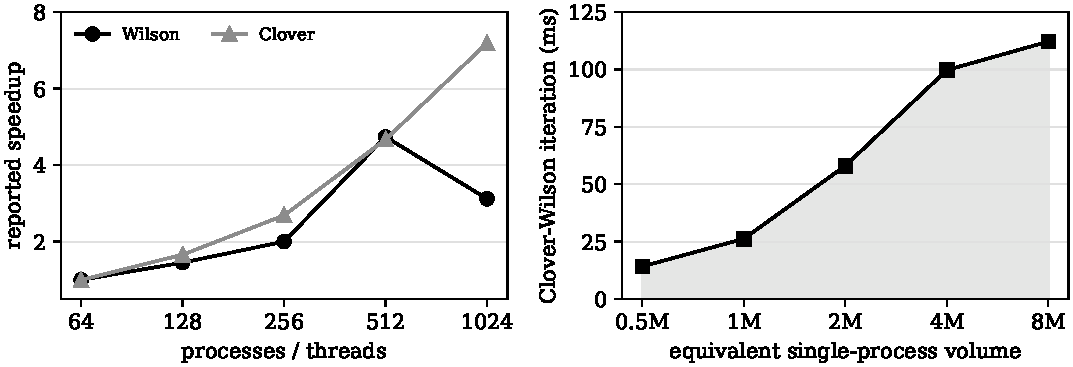
\includegraphics[width=0.94\textwidth,height=0.55\textheight,keepaspectratio]
  {High-Performance_Implementation_MG_assets/paper_assets/fig_508_scaling.pdf}
  \par{\small 图 7：TEST8 c64 强扩展与 1024-rank 双精度对照。}
  \par\vspace{0.04cm}
  {\scriptsize 64 卡池容量估算 \(\approx2048\) GiB 来自 TEST8 原始表；
  1024 是 MPI rank/thread 规模，不是 1024 张 GPU 的实测聚合性能。\par}
\end{frame}

\begin{frame}[plain]
  \vfill
  \centering
  {\usebeamerfont{title}\usebeamercolor[fg]{title}
  \Huge\bfseries 谢谢\par}
  \vspace{0.7cm}
  {\Large PyQCU Strict MultiGrid\par}
  \vspace{0.5cm}
  {\large 下一步：粗层同步、通信重叠和 setup 显存做成可复验收益。\par}
  \vspace{1.0cm}
  \small
  \url{https://github.com/zhangxin8069/PyQCU}\\
  数据基线：\code{git tag test27}\\[0.5cm]
  \textcolor{coral}{\bfseries Q \& A}
\end{frame}

\end{document}
